\documentclass[1p]{elsarticle_modified}
%\bibliographystyle{elsarticle-num}

%\usepackage[colorlinks]{hyperref}
%\usepackage{abbrmath_seonhwa} %\Abb, \Ascr, \Acal ,\Abf, \Afrak
\usepackage{amsfonts}
\usepackage{amssymb}
\usepackage{amsmath}
\usepackage{amsthm}
\usepackage{scalefnt}
\usepackage{amsbsy}
\usepackage{kotex}
\usepackage{caption}
\usepackage{subfig}
\usepackage{color}
\usepackage{graphicx}
\usepackage{xcolor} %% white, black, red, green, blue, cyan, magenta, yellow
\usepackage{float}
\usepackage{setspace}
\usepackage{hyperref}

\usepackage{tikz}
\usetikzlibrary{arrows}

\usepackage{multirow}
\usepackage{array} % fixed length table
\usepackage{hhline}

%%%%%%%%%%%%%%%%%%%%%
\makeatletter
\renewcommand*\env@matrix[1][\arraystretch]{%
	\edef\arraystretch{#1}%
	\hskip -\arraycolsep
	\let\@ifnextchar\new@ifnextchar
	\array{*\c@MaxMatrixCols c}}
\makeatother %https://tex.stackexchange.com/questions/14071/how-can-i-increase-the-line-spacing-in-a-matrix
%%%%%%%%%%%%%%%

\usepackage[normalem]{ulem}

\newcommand{\msout}[1]{\ifmmode\text{\sout{\ensuremath{#1}}}\else\sout{#1}\fi}
%SOURCE: \msout is \stkout macro in https://tex.stackexchange.com/questions/20609/strikeout-in-math-mode

\newcommand{\cancel}[1]{
	\ifmmode
	{\color{red}\msout{#1}}
	\else
	{\color{red}\sout{#1}}
	\fi
}

\newcommand{\add}[1]{
	{\color{blue}\uwave{#1}}
}

\newcommand{\replace}[2]{
	\ifmmode
	{\color{red}\msout{#1}}{\color{blue}\uwave{#2}}
	\else
	{\color{red}\sout{#1}}{\color{blue}\uwave{#2}}
	\fi
}

\newcommand{\Sol}{\mathcal{S}} %segment
\newcommand{\D}{D} %diagram
\newcommand{\A}{\mathcal{A}} %arc


%%%%%%%%%%%%%%%%%%%%%%%%%%%%%5 test

\def\sl{\operatorname{\textup{SL}}(2,\Cbb)}
\def\psl{\operatorname{\textup{PSL}}(2,\Cbb)}
\def\quan{\mkern 1mu \triangleright \mkern 1mu}

\theoremstyle{definition}
\newtheorem{thm}{Theorem}[section]
\newtheorem{prop}[thm]{Proposition}
\newtheorem{lem}[thm]{Lemma}
\newtheorem{ques}[thm]{Question}
\newtheorem{cor}[thm]{Corollary}
\newtheorem{defn}[thm]{Definition}
\newtheorem{exam}[thm]{Example}
\newtheorem{rmk}[thm]{Remark}
\newtheorem{alg}[thm]{Algorithm}

\newcommand{\I}{\sqrt{-1}}
\begin{document}

%\begin{frontmatter}
%
%\title{Boundary parabolic representations of knots up to 8 crossings}
%
%%% Group authors per affiliation:
%\author{Yunhi Cho} 
%\address{Department of Mathematics, University of Seoul, Seoul, Korea}
%\ead{yhcho@uos.ac.kr}
%
%
%\author{Seonhwa Kim} %\fnref{s_kim}}
%\address{Center for Geometry and Physics, Institute for Basic Science, Pohang, 37673, Korea}
%\ead{ryeona17@ibs.re.kr}
%
%\author{Hyuk Kim}
%\address{Department of Mathematical Sciences, Seoul National University, Seoul 08826, Korea}
%\ead{hyukkim@snu.ac.kr}
%
%\author{Seokbeom Yoon}
%\address{Department of Mathematical Sciences, Seoul National University, Seoul, 08826,  Korea}
%\ead{sbyoon15@snu.ac.kr}
%
%\begin{abstract}
%We find all boundary parabolic representation of knots up to 8 crossings.
%
%\end{abstract}
%\begin{keyword}
%    \MSC[2010] 57M25 
%\end{keyword}
%
%\end{frontmatter}

%\linenumbers
%\tableofcontents
%
\newcommand\colored[1]{\textcolor{white}{\rule[-0.35ex]{0.8em}{1.4ex}}\kern-0.8em\color{red} #1}%
%\newcommand\colored[1]{\textcolor{white}{ #1}\kern-2.17ex	\textcolor{white}{ #1}\kern-1.81ex	\textcolor{white}{ #1}\kern-2.15ex\color{red}#1	}

{\Large $\underline{12a_{0782}~(K12a_{0782})}$}

\setlength{\tabcolsep}{10pt}
\renewcommand{\arraystretch}{1.6}
\vspace{1cm}\begin{tabular}{m{100pt}>{\centering\arraybackslash}m{274pt}}
\multirow{5}{120pt}{
	\centering
	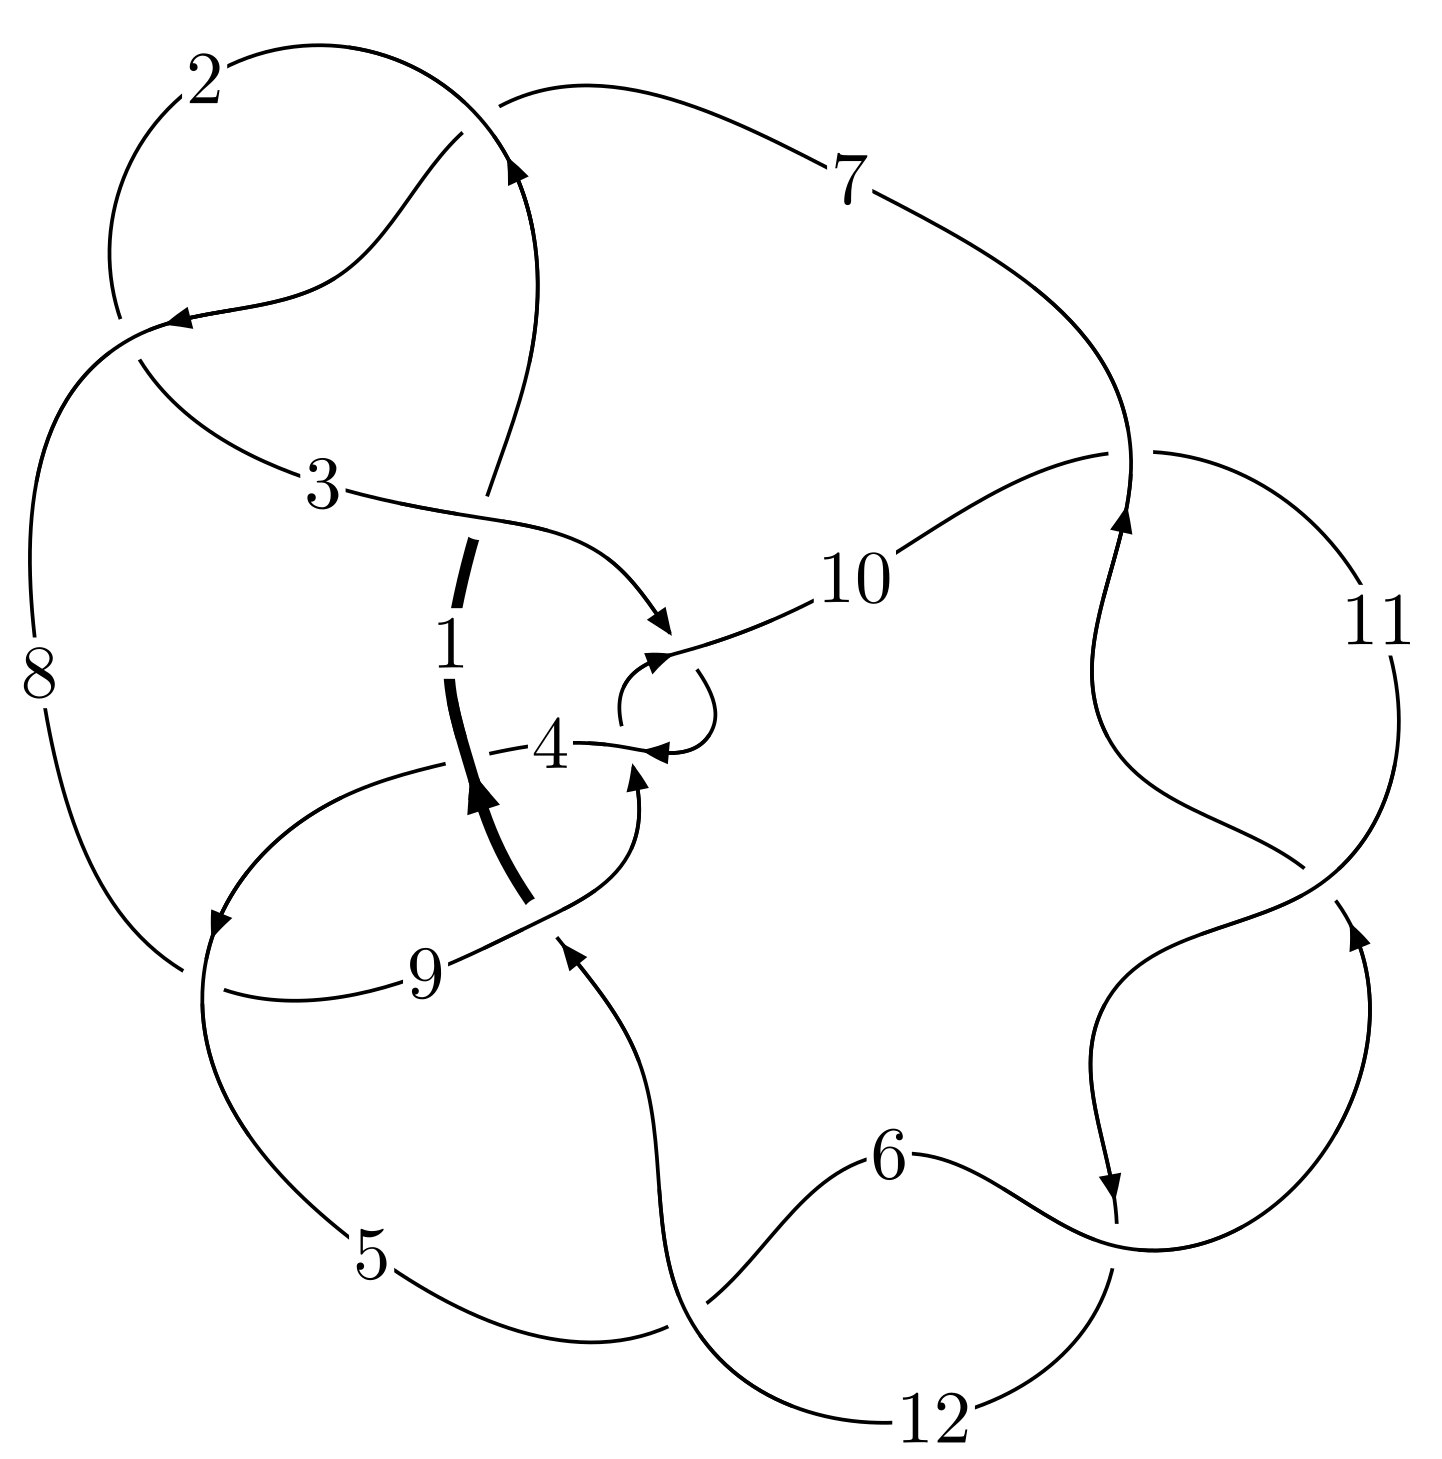
\includegraphics[width=112pt]{../../../GIT/diagram.site/Diagrams/png/1583_12a_0782.png}\\
\ \ \ A knot diagram\footnotemark}&
\allowdisplaybreaks
\textbf{Linearized knot diagam} \\
\cline{2-2}
 &
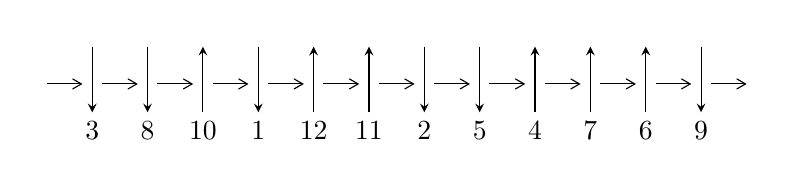
\begin{tikzpicture}[x=20pt, y=17pt]
	% nodes
	\node (C0) at (0, 0) {};
	\node (C1) at (1, 0) {};
	\node (C1U) at (1, +1) {};
	\node (C1D) at (1, -1) {3};

	\node (C2) at (2, 0) {};
	\node (C2U) at (2, +1) {};
	\node (C2D) at (2, -1) {8};

	\node (C3) at (3, 0) {};
	\node (C3U) at (3, +1) {};
	\node (C3D) at (3, -1) {10};

	\node (C4) at (4, 0) {};
	\node (C4U) at (4, +1) {};
	\node (C4D) at (4, -1) {1};

	\node (C5) at (5, 0) {};
	\node (C5U) at (5, +1) {};
	\node (C5D) at (5, -1) {12};

	\node (C6) at (6, 0) {};
	\node (C6U) at (6, +1) {};
	\node (C6D) at (6, -1) {11};

	\node (C7) at (7, 0) {};
	\node (C7U) at (7, +1) {};
	\node (C7D) at (7, -1) {2};

	\node (C8) at (8, 0) {};
	\node (C8U) at (8, +1) {};
	\node (C8D) at (8, -1) {5};

	\node (C9) at (9, 0) {};
	\node (C9U) at (9, +1) {};
	\node (C9D) at (9, -1) {4};

	\node (C10) at (10, 0) {};
	\node (C10U) at (10, +1) {};
	\node (C10D) at (10, -1) {7};

	\node (C11) at (11, 0) {};
	\node (C11U) at (11, +1) {};
	\node (C11D) at (11, -1) {6};

	\node (C12) at (12, 0) {};
	\node (C12U) at (12, +1) {};
	\node (C12D) at (12, -1) {9};
	\node (C13) at (13, 0) {};

	% arrows
	\draw[->,>={angle 60}]
	(C0) edge (C1) (C1) edge (C2) (C2) edge (C3) (C3) edge (C4) (C4) edge (C5) (C5) edge (C6) (C6) edge (C7) (C7) edge (C8) (C8) edge (C9) (C9) edge (C10) (C10) edge (C11) (C11) edge (C12) (C12) edge (C13) ;	\draw[->,>=stealth]
	(C1U) edge (C1D) (C2U) edge (C2D) (C3D) edge (C3U) (C4U) edge (C4D) (C5D) edge (C5U) (C6D) edge (C6U) (C7U) edge (C7D) (C8U) edge (C8D) (C9D) edge (C9U) (C10D) edge (C10U) (C11D) edge (C11U) (C12U) edge (C12D) ;
	\end{tikzpicture} \\
\hhline{~~} \\& 
\textbf{Solving Sequence} \\ \cline{2-2} 
 &
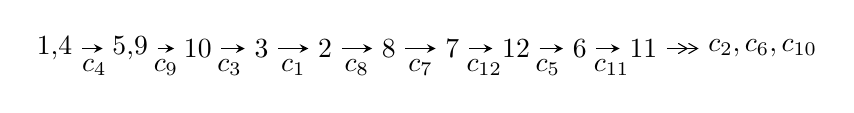
\begin{tikzpicture}[x=23pt, y=7pt]
	% node
	\node (A0) at (-1/8, 0) {1,4};
	\node (A1) at (17/16, 0) {5,9};
	\node (A2) at (17/8, 0) {10};
	\node (A3) at (25/8, 0) {3};
	\node (A4) at (33/8, 0) {2};
	\node (A5) at (41/8, 0) {8};
	\node (A6) at (49/8, 0) {7};
	\node (A7) at (57/8, 0) {12};
	\node (A8) at (65/8, 0) {6};
	\node (A9) at (73/8, 0) {11};
	\node (C1) at (1/2, -1) {$c_{4}$};
	\node (C2) at (13/8, -1) {$c_{9}$};
	\node (C3) at (21/8, -1) {$c_{3}$};
	\node (C4) at (29/8, -1) {$c_{1}$};
	\node (C5) at (37/8, -1) {$c_{8}$};
	\node (C6) at (45/8, -1) {$c_{7}$};
	\node (C7) at (53/8, -1) {$c_{12}$};
	\node (C8) at (61/8, -1) {$c_{5}$};
	\node (C9) at (69/8, -1) {$c_{11}$};
	\node (A10) at (11, 0) {$c_{2},c_{6},c_{10}$};

	% edge
	\draw[->,>=stealth]	
	(A0) edge (A1) (A1) edge (A2) (A2) edge (A3) (A3) edge (A4) (A4) edge (A5) (A5) edge (A6) (A6) edge (A7) (A7) edge (A8) (A8) edge (A9) ;
	\draw[->>,>={angle 60}]	
	(A9) edge (A10);
\end{tikzpicture} \\ 

\end{tabular} \\

\footnotetext{
The image of knot diagram is generated by the software ``\textbf{Draw programme}" developed by Andrew Bartholomew(\url{http://www.layer8.co.uk/maths/draw/index.htm\#Running-draw}), where we modified some parts for our purpose(\url{https://github.com/CATsTAILs/LinksPainter}).
}\phantom \\ \newline 
\centering \textbf{Ideals for irreducible components\footnotemark of $X_{\text{par}}$} 
 
\begin{align*}
I^u_{1}&=\langle 
2.11865\times10^{428} u^{94}-1.08212\times10^{429} u^{93}+\cdots+2.38307\times10^{427} b+9.28828\times10^{427},\\
\phantom{I^u_{1}}&\phantom{= \langle  }3.77418\times10^{428} u^{94}-2.18208\times10^{429} u^{93}+\cdots+2.38307\times10^{427} a+4.03773\times10^{428},\;u^{95}-6 u^{94}+\cdots-30 u+1\rangle \\
I^u_{2}&=\langle 
-26712 u^{19}-136095 u^{18}+\cdots+41267 b+19242,\\
\phantom{I^u_{2}}&\phantom{= \langle  }-97076 u^{19}-295395 u^{18}+\cdots+41267 a+23990,\;u^{20}+3 u^{19}+\cdots-3 u^3+1\rangle \\
\\
\end{align*}
\raggedright * 2 irreducible components of $\dim_{\mathbb{C}}=0$, with total 115 representations.\\
\footnotetext{All coefficients of polynomials are rational numbers. But the coefficients are sometimes approximated in decimal forms when there is not enough margin.}
\newpage
\renewcommand{\arraystretch}{1}
\centering \section*{I. $I^u_{1}= \langle 2.12\times10^{428} u^{94}-1.08\times10^{429} u^{93}+\cdots+2.38\times10^{427} b+9.29\times10^{427},\;3.77\times10^{428} u^{94}-2.18\times10^{429} u^{93}+\cdots+2.38\times10^{427} a+4.04\times10^{428},\;u^{95}-6 u^{94}+\cdots-30 u+1 \rangle$}
\flushleft \textbf{(i) Arc colorings}\\
\begin{tabular}{m{7pt} m{180pt} m{7pt} m{180pt} }
\flushright $a_{1}=$&$\begin{pmatrix}0\\u\end{pmatrix}$ \\
\flushright $a_{4}=$&$\begin{pmatrix}1\\0\end{pmatrix}$ \\
\flushright $a_{5}=$&$\begin{pmatrix}1\\u^2\end{pmatrix}$ \\
\flushright $a_{9}=$&$\begin{pmatrix}-15.8375 u^{94}+91.5658 u^{93}+\cdots+24.0389 u-16.9434\\-8.89041 u^{94}+45.4085 u^{93}+\cdots+72.2169 u-3.89761\end{pmatrix}$ \\
\flushright $a_{10}=$&$\begin{pmatrix}-24.7279 u^{94}+136.974 u^{93}+\cdots+96.2557 u-20.8410\\-8.89041 u^{94}+45.4085 u^{93}+\cdots+72.2169 u-3.89761\end{pmatrix}$ \\
\flushright $a_{3}=$&$\begin{pmatrix}6.52903 u^{94}-30.9088 u^{93}+\cdots-1287.55 u+60.5572\\4.24134 u^{94}-26.0490 u^{93}+\cdots+899.845 u-36.4157\end{pmatrix}$ \\
\flushright $a_{2}=$&$\begin{pmatrix}45.2454 u^{94}-254.396 u^{93}+\cdots+3003.20 u-103.906\\20.5669 u^{94}-115.764 u^{93}+\cdots+1600.35 u-58.5354\end{pmatrix}$ \\
\flushright $a_{8}=$&$\begin{pmatrix}-25.8044 u^{94}+142.203 u^{93}+\cdots+184.186 u-24.2999\\-14.1864 u^{94}+74.6594 u^{93}+\cdots-192.744 u+5.26665\end{pmatrix}$ \\
\flushright $a_{7}=$&$\begin{pmatrix}17.4039 u^{94}-102.619 u^{93}+\cdots+3770.93 u-153.901\\35.8133 u^{94}-200.858 u^{93}+\cdots+2303.55 u-81.5877\end{pmatrix}$ \\
\flushright $a_{12}=$&$\begin{pmatrix}61.6817 u^{94}-355.931 u^{93}+\cdots+5974.92 u-220.895\\8.86630 u^{94}-48.4230 u^{93}+\cdots+165.604 u-2.28769\end{pmatrix}$ \\
\flushright $a_{6}=$&$\begin{pmatrix}9.50913 u^{94}-73.9815 u^{93}+\cdots+6807.32 u-286.013\\5.28830 u^{94}-29.8106 u^{93}+\cdots+261.607 u-7.96118\end{pmatrix}$ \\
\flushright $a_{11}=$&$\begin{pmatrix}-135.721 u^{94}+772.386 u^{93}+\cdots-9767.50 u+335.007\\-17.0754 u^{94}+96.2722 u^{93}+\cdots-790.075 u+25.1554\end{pmatrix}$\\&\end{tabular}
\flushleft \textbf{(ii) Obstruction class $= -1$}\\~\\
\flushleft \textbf{(iii) Cusp Shapes $= 59.3924 u^{94}-339.420 u^{93}+\cdots+6474.19 u-259.078$}\\~\\
\newpage\renewcommand{\arraystretch}{1}
\flushleft \textbf{(iv) u-Polynomials at the component}\newline \\
\begin{tabular}{m{50pt}|m{274pt}}
Crossings & \hspace{64pt}u-Polynomials at each crossing \\
\hline $$\begin{aligned}c_{1}\end{aligned}$$&$\begin{aligned}
&u^{95}+47 u^{94}+\cdots+22027 u+1849
\end{aligned}$\\
\hline $$\begin{aligned}c_{2},c_{7}\end{aligned}$$&$\begin{aligned}
&u^{95}+u^{94}+\cdots+107 u+43
\end{aligned}$\\
\hline $$\begin{aligned}c_{3},c_{9}\end{aligned}$$&$\begin{aligned}
&u^{95}+u^{94}+\cdots+3057 u+677
\end{aligned}$\\
\hline $$\begin{aligned}c_{4}\end{aligned}$$&$\begin{aligned}
&u^{95}-6 u^{94}+\cdots-30 u+1
\end{aligned}$\\
\hline $$\begin{aligned}c_{5},c_{6},c_{10}\\c_{11}\end{aligned}$$&$\begin{aligned}
&u^{95}- u^{94}+\cdots+378 u+43
\end{aligned}$\\
\hline $$\begin{aligned}c_{8}\end{aligned}$$&$\begin{aligned}
&u^{95}+4 u^{94}+\cdots+2534 u+649
\end{aligned}$\\
\hline $$\begin{aligned}c_{12}\end{aligned}$$&$\begin{aligned}
&u^{95}+3 u^{94}+\cdots-54430 u-10639
\end{aligned}$\\
\hline
\end{tabular}\\~\\
\newpage\renewcommand{\arraystretch}{1}
\flushleft \textbf{(v) Riley Polynomials at the component}\newline \\
\begin{tabular}{m{50pt}|m{274pt}}
Crossings & \hspace{64pt}Riley Polynomials at each crossing \\
\hline $$\begin{aligned}c_{1}\end{aligned}$$&$\begin{aligned}
&y^{95}+13 y^{94}+\cdots-54944849 y-3418801
\end{aligned}$\\
\hline $$\begin{aligned}c_{2},c_{7}\end{aligned}$$&$\begin{aligned}
&y^{95}-47 y^{94}+\cdots+22027 y-1849
\end{aligned}$\\
\hline $$\begin{aligned}c_{3},c_{9}\end{aligned}$$&$\begin{aligned}
&y^{95}+75 y^{94}+\cdots-16234519 y-458329
\end{aligned}$\\
\hline $$\begin{aligned}c_{4}\end{aligned}$$&$\begin{aligned}
&y^{95}-8 y^{94}+\cdots+30 y-1
\end{aligned}$\\
\hline $$\begin{aligned}c_{5},c_{6},c_{10}\\c_{11}\end{aligned}$$&$\begin{aligned}
&y^{95}+119 y^{94}+\cdots-54314 y-1849
\end{aligned}$\\
\hline $$\begin{aligned}c_{8}\end{aligned}$$&$\begin{aligned}
&y^{95}-24 y^{94}+\cdots+11018672 y-421201
\end{aligned}$\\
\hline $$\begin{aligned}c_{12}\end{aligned}$$&$\begin{aligned}
&y^{95}-41 y^{94}+\cdots+5892243774 y-113188321
\end{aligned}$\\
\hline
\end{tabular}\\~\\
\newpage\flushleft \textbf{(vi) Complex Volumes and Cusp Shapes}
$$\begin{array}{c|c|c}  
\text{Solutions to }I^u_{1}& \I (\text{vol} + \sqrt{-1}CS) & \text{Cusp shape}\\
 \hline 
\begin{aligned}
u &= -0.289117 + 0.959904 I \\
a &= \phantom{-}0.247983 - 0.890243 I \\
b &= -0.444716 + 0.246446 I\end{aligned}
 & -0.95680 + 2.64726 I & \phantom{-0.000000 } 0 \\ \hline\begin{aligned}
u &= -0.289117 - 0.959904 I \\
a &= \phantom{-}0.247983 + 0.890243 I \\
b &= -0.444716 - 0.246446 I\end{aligned}
 & -0.95680 - 2.64726 I & \phantom{-0.000000 } 0 \\ \hline\begin{aligned}
u &= \phantom{-}0.994310 + 0.055911 I \\
a &= \phantom{-}0.783766 - 0.213159 I \\
b &= -0.87312 + 1.52848 I\end{aligned}
 & -13.5623 - 6.1465 I & \phantom{-0.000000 } 0 \\ \hline\begin{aligned}
u &= \phantom{-}0.994310 - 0.055911 I \\
a &= \phantom{-}0.783766 + 0.213159 I \\
b &= -0.87312 - 1.52848 I\end{aligned}
 & -13.5623 + 6.1465 I & \phantom{-0.000000 } 0 \\ \hline\begin{aligned}
u &= -0.720342 + 0.734951 I \\
a &= \phantom{-}1.182430 + 0.140111 I \\
b &= -1.49757 - 0.03566 I\end{aligned}
 & -9.78510 + 9.45959 I & \phantom{-0.000000 } 0 \\ \hline\begin{aligned}
u &= -0.720342 - 0.734951 I \\
a &= \phantom{-}1.182430 - 0.140111 I \\
b &= -1.49757 + 0.03566 I\end{aligned}
 & -9.78510 - 9.45959 I & \phantom{-0.000000 } 0 \\ \hline\begin{aligned}
u &= -0.964676 + 0.376723 I \\
a &= \phantom{-}0.691405 + 0.116066 I \\
b &= -0.522740 - 1.139190 I\end{aligned}
 & -3.29940 + 0.97709 I & \phantom{-0.000000 } 0 \\ \hline\begin{aligned}
u &= -0.964676 - 0.376723 I \\
a &= \phantom{-}0.691405 - 0.116066 I \\
b &= -0.522740 + 1.139190 I\end{aligned}
 & -3.29940 - 0.97709 I & \phantom{-0.000000 } 0 \\ \hline\begin{aligned}
u &= -0.460088 + 0.936654 I \\
a &= -0.477266 + 1.215140 I \\
b &= \phantom{-}0.745588 - 0.483057 I\end{aligned}
 & -9.39170 + 3.08813 I & \phantom{-0.000000 } 0 \\ \hline\begin{aligned}
u &= -0.460088 - 0.936654 I \\
a &= -0.477266 - 1.215140 I \\
b &= \phantom{-}0.745588 + 0.483057 I\end{aligned}
 & -9.39170 - 3.08813 I & \phantom{-0.000000 } 0\\
 \hline 
 \end{array}$$\newpage$$\begin{array}{c|c|c}  
\text{Solutions to }I^u_{1}& \I (\text{vol} + \sqrt{-1}CS) & \text{Cusp shape}\\
 \hline 
\begin{aligned}
u &= \phantom{-}0.904927 + 0.274763 I \\
a &= \phantom{-}1.023640 + 0.473666 I \\
b &= -0.567159 + 1.166250 I\end{aligned}
 & -3.73367 - 3.88567 I & \phantom{-0.000000 } 0 \\ \hline\begin{aligned}
u &= \phantom{-}0.904927 - 0.274763 I \\
a &= \phantom{-}1.023640 - 0.473666 I \\
b &= -0.567159 - 1.166250 I\end{aligned}
 & -3.73367 + 3.88567 I & \phantom{-0.000000 } 0 \\ \hline\begin{aligned}
u &= -1.035510 + 0.231678 I \\
a &= \phantom{-}0.861175 + 1.081130 I \\
b &= \phantom{-}0.327085 + 0.335473 I\end{aligned}
 & -11.24410 - 5.06256 I & \phantom{-0.000000 } 0 \\ \hline\begin{aligned}
u &= -1.035510 - 0.231678 I \\
a &= \phantom{-}0.861175 - 1.081130 I \\
b &= \phantom{-}0.327085 - 0.335473 I\end{aligned}
 & -11.24410 + 5.06256 I & \phantom{-0.000000 } 0 \\ \hline\begin{aligned}
u &= -0.668864 + 0.829081 I \\
a &= -0.984513 - 0.209552 I \\
b &= \phantom{-}1.202030 + 0.080693 I\end{aligned}
 & -0.93766 + 7.51485 I & \phantom{-0.000000 } 0 \\ \hline\begin{aligned}
u &= -0.668864 - 0.829081 I \\
a &= -0.984513 + 0.209552 I \\
b &= \phantom{-}1.202030 - 0.080693 I\end{aligned}
 & -0.93766 - 7.51485 I & \phantom{-0.000000 } 0 \\ \hline\begin{aligned}
u &= \phantom{-}0.927854 + 0.110516 I \\
a &= -0.751235 - 0.065614 I \\
b &= \phantom{-}0.73470 - 1.39916 I\end{aligned}
 & -5.20284 - 5.28701 I & \phantom{-0.000000 } 0 \\ \hline\begin{aligned}
u &= \phantom{-}0.927854 - 0.110516 I \\
a &= -0.751235 + 0.065614 I \\
b &= \phantom{-}0.73470 + 1.39916 I\end{aligned}
 & -5.20284 + 5.28701 I & \phantom{-0.000000 } 0 \\ \hline\begin{aligned}
u &= -0.958848 + 0.490910 I \\
a &= -0.934638 + 0.178527 I \\
b &= \phantom{-}0.903421 + 0.646140 I\end{aligned}
 & -3.06403 + 1.76286 I & \phantom{-0.000000 } 0 \\ \hline\begin{aligned}
u &= -0.958848 - 0.490910 I \\
a &= -0.934638 - 0.178527 I \\
b &= \phantom{-}0.903421 - 0.646140 I\end{aligned}
 & -3.06403 - 1.76286 I & \phantom{-0.000000 } 0\\
 \hline 
 \end{array}$$\newpage$$\begin{array}{c|c|c}  
\text{Solutions to }I^u_{1}& \I (\text{vol} + \sqrt{-1}CS) & \text{Cusp shape}\\
 \hline 
\begin{aligned}
u &= -0.345722 + 0.851089 I \\
a &= -1.033130 - 0.722887 I \\
b &= \phantom{-}0.456443 + 0.763853 I\end{aligned}
 & \phantom{-}0.13024 + 2.18300 I & \phantom{-0.000000 } 0 \\ \hline\begin{aligned}
u &= -0.345722 - 0.851089 I \\
a &= -1.033130 + 0.722887 I \\
b &= \phantom{-}0.456443 - 0.763853 I\end{aligned}
 & \phantom{-}0.13024 - 2.18300 I & \phantom{-0.000000 } 0 \\ \hline\begin{aligned}
u &= -0.280938 + 1.045430 I \\
a &= \phantom{-}0.66353 + 1.42921 I \\
b &= -0.109739 - 0.905737 I\end{aligned}
 & -0.03198 + 3.42317 I & \phantom{-0.000000 } 0 \\ \hline\begin{aligned}
u &= -0.280938 - 1.045430 I \\
a &= \phantom{-}0.66353 - 1.42921 I \\
b &= -0.109739 + 0.905737 I\end{aligned}
 & -0.03198 - 3.42317 I & \phantom{-0.000000 } 0 \\ \hline\begin{aligned}
u &= \phantom{-}0.292505 + 0.842148 I \\
a &= -0.839759 + 0.369119 I \\
b &= \phantom{-}0.760407 + 0.174654 I\end{aligned}
 & \phantom{-}2.37641 + 0.47115 I & \phantom{-0.000000 } 0 \\ \hline\begin{aligned}
u &= \phantom{-}0.292505 - 0.842148 I \\
a &= -0.839759 - 0.369119 I \\
b &= \phantom{-}0.760407 - 0.174654 I\end{aligned}
 & \phantom{-}2.37641 - 0.47115 I & \phantom{-0.000000 } 0 \\ \hline\begin{aligned}
u &= -1.065600 + 0.308081 I \\
a &= -0.679248 - 0.343845 I \\
b &= \phantom{-}0.59924 + 1.40120 I\end{aligned}
 & -11.60630 + 0.90409 I & \phantom{-0.000000 } 0 \\ \hline\begin{aligned}
u &= -1.065600 - 0.308081 I \\
a &= -0.679248 + 0.343845 I \\
b &= \phantom{-}0.59924 - 1.40120 I\end{aligned}
 & -11.60630 - 0.90409 I & \phantom{-0.000000 } 0 \\ \hline\begin{aligned}
u &= -0.883069\phantom{ +0.000000I} \\
a &= \phantom{-}0.647690\phantom{ +0.000000I} \\
b &= -0.352931\phantom{ +0.000000I}\end{aligned}
 & -1.80352\phantom{ +0.000000I} & \phantom{-0.000000 } 0 \\ \hline\begin{aligned}
u &= \phantom{-}0.671202 + 0.561115 I \\
a &= -1.45085 + 0.08625 I \\
b &= \phantom{-}1.116020 + 0.035605 I\end{aligned}
 & -7.48014 - 4.78255 I & \phantom{-0.000000 } 0\\
 \hline 
 \end{array}$$\newpage$$\begin{array}{c|c|c}  
\text{Solutions to }I^u_{1}& \I (\text{vol} + \sqrt{-1}CS) & \text{Cusp shape}\\
 \hline 
\begin{aligned}
u &= \phantom{-}0.671202 - 0.561115 I \\
a &= -1.45085 - 0.08625 I \\
b &= \phantom{-}1.116020 - 0.035605 I\end{aligned}
 & -7.48014 + 4.78255 I & \phantom{-0.000000 } 0 \\ \hline\begin{aligned}
u &= -0.259215 + 1.102920 I \\
a &= -0.67085 - 1.72442 I \\
b &= \phantom{-}0.078689 + 1.097050 I\end{aligned}
 & -7.87333 + 3.80259 I & \phantom{-0.000000 } 0 \\ \hline\begin{aligned}
u &= -0.259215 - 1.102920 I \\
a &= -0.67085 + 1.72442 I \\
b &= \phantom{-}0.078689 - 1.097050 I\end{aligned}
 & -7.87333 - 3.80259 I & \phantom{-0.000000 } 0 \\ \hline\begin{aligned}
u &= -0.586307 + 0.973561 I \\
a &= \phantom{-}0.695896 + 0.316974 I \\
b &= -0.745228 - 0.093350 I\end{aligned}
 & \phantom{-}1.69308 + 4.33267 I & \phantom{-0.000000 } 0 \\ \hline\begin{aligned}
u &= -0.586307 - 0.973561 I \\
a &= \phantom{-}0.695896 - 0.316974 I \\
b &= -0.745228 + 0.093350 I\end{aligned}
 & \phantom{-}1.69308 - 4.33267 I & \phantom{-0.000000 } 0 \\ \hline\begin{aligned}
u &= -0.983002 + 0.573098 I \\
a &= \phantom{-}1.138440 - 0.219507 I \\
b &= -1.173070 - 0.648972 I\end{aligned}
 & -11.15500 + 2.05012 I & \phantom{-0.000000 } 0 \\ \hline\begin{aligned}
u &= -0.983002 - 0.573098 I \\
a &= \phantom{-}1.138440 + 0.219507 I \\
b &= -1.173070 + 0.648972 I\end{aligned}
 & -11.15500 - 2.05012 I & \phantom{-0.000000 } 0 \\ \hline\begin{aligned}
u &= \phantom{-}1.110710 + 0.290968 I \\
a &= -1.135840 - 0.546865 I \\
b &= \phantom{-}0.390635 - 0.902935 I\end{aligned}
 & -9.35548 - 3.78734 I & \phantom{-0.000000 } 0 \\ \hline\begin{aligned}
u &= \phantom{-}1.110710 - 0.290968 I \\
a &= -1.135840 + 0.546865 I \\
b &= \phantom{-}0.390635 + 0.902935 I\end{aligned}
 & -9.35548 + 3.78734 I & \phantom{-0.000000 } 0 \\ \hline\begin{aligned}
u &= -1.152000 + 0.039647 I \\
a &= -0.722058 - 0.475056 I \\
b &= -0.076023 - 0.384783 I\end{aligned}
 & -3.37674 - 2.78375 I & \phantom{-0.000000 } 0\\
 \hline 
 \end{array}$$\newpage$$\begin{array}{c|c|c}  
\text{Solutions to }I^u_{1}& \I (\text{vol} + \sqrt{-1}CS) & \text{Cusp shape}\\
 \hline 
\begin{aligned}
u &= -1.152000 - 0.039647 I \\
a &= -0.722058 + 0.475056 I \\
b &= -0.076023 + 0.384783 I\end{aligned}
 & -3.37674 + 2.78375 I & \phantom{-0.000000 } 0 \\ \hline\begin{aligned}
u &= \phantom{-}0.501415 + 0.649342 I \\
a &= \phantom{-}1.240930 - 0.257663 I \\
b &= -0.968639 - 0.104841 I\end{aligned}
 & \phantom{-}0.59827 - 2.85627 I & \phantom{-0.000000 } 0 \\ \hline\begin{aligned}
u &= \phantom{-}0.501415 - 0.649342 I \\
a &= \phantom{-}1.240930 + 0.257663 I \\
b &= -0.968639 + 0.104841 I\end{aligned}
 & \phantom{-}0.59827 + 2.85627 I & \phantom{-0.000000 } 0 \\ \hline\begin{aligned}
u &= \phantom{-}0.971469 + 0.866417 I \\
a &= \phantom{-}1.43450 - 0.30255 I \\
b &= -0.28159 + 1.42485 I\end{aligned}
 & -18.0405 - 6.3079 I & \phantom{-0.000000 } 0 \\ \hline\begin{aligned}
u &= \phantom{-}0.971469 - 0.866417 I \\
a &= \phantom{-}1.43450 + 0.30255 I \\
b &= -0.28159 - 1.42485 I\end{aligned}
 & -18.0405 + 6.3079 I & \phantom{-0.000000 } 0 \\ \hline\begin{aligned}
u &= \phantom{-}1.076390 + 0.734224 I \\
a &= -1.213520 + 0.008244 I \\
b &= \phantom{-}0.246608 - 1.273080 I\end{aligned}
 & -8.70092 - 4.69865 I & \phantom{-0.000000 } 0 \\ \hline\begin{aligned}
u &= \phantom{-}1.076390 - 0.734224 I \\
a &= -1.213520 - 0.008244 I \\
b &= \phantom{-}0.246608 + 1.273080 I\end{aligned}
 & -8.70092 + 4.69865 I & \phantom{-0.000000 } 0 \\ \hline\begin{aligned}
u &= \phantom{-}0.005021 + 0.677987 I \\
a &= \phantom{-}2.14658 + 1.03569 I \\
b &= -0.504060 - 0.709244 I\end{aligned}
 & -6.31275 + 2.09871 I & \phantom{-}0.46926 - 2.25158 I \\ \hline\begin{aligned}
u &= \phantom{-}0.005021 - 0.677987 I \\
a &= \phantom{-}2.14658 - 1.03569 I \\
b &= -0.504060 + 0.709244 I\end{aligned}
 & -6.31275 - 2.09871 I & \phantom{-}0.46926 + 2.25158 I \\ \hline\begin{aligned}
u &= \phantom{-}0.426863 + 0.431697 I \\
a &= -2.28395 - 2.76519 I \\
b &= \phantom{-}0.469197 - 1.010660 I\end{aligned}
 & -10.94880 - 7.65283 I & -5.22797 + 11.06490 I\\
 \hline 
 \end{array}$$\newpage$$\begin{array}{c|c|c}  
\text{Solutions to }I^u_{1}& \I (\text{vol} + \sqrt{-1}CS) & \text{Cusp shape}\\
 \hline 
\begin{aligned}
u &= \phantom{-}0.426863 - 0.431697 I \\
a &= -2.28395 + 2.76519 I \\
b &= \phantom{-}0.469197 + 1.010660 I\end{aligned}
 & -10.94880 + 7.65283 I & -5.22797 - 11.06490 I \\ \hline\begin{aligned}
u &= -0.57480 + 1.29543 I \\
a &= \phantom{-}0.450516 + 0.332022 I \\
b &= -0.416072 - 1.184950 I\end{aligned}
 & -4.33687 + 0.29946 I & \phantom{-0.000000 } 0 \\ \hline\begin{aligned}
u &= -0.57480 - 1.29543 I \\
a &= \phantom{-}0.450516 - 0.332022 I \\
b &= -0.416072 + 1.184950 I\end{aligned}
 & -4.33687 - 0.29946 I & \phantom{-0.000000 } 0 \\ \hline\begin{aligned}
u &= \phantom{-}0.481464 + 0.319780 I \\
a &= \phantom{-}0.89697 + 2.60290 I \\
b &= -0.359298 + 1.076130 I\end{aligned}
 & -3.23096 - 6.09113 I & -3.77113 + 12.10008 I \\ \hline\begin{aligned}
u &= \phantom{-}0.481464 - 0.319780 I \\
a &= \phantom{-}0.89697 - 2.60290 I \\
b &= -0.359298 - 1.076130 I\end{aligned}
 & -3.23096 + 6.09113 I & -3.77113 - 12.10008 I \\ \hline\begin{aligned}
u &= -0.16641 + 1.41807 I \\
a &= \phantom{-}0.098862 - 0.226912 I \\
b &= -0.161596 - 0.347833 I\end{aligned}
 & -1.34120 + 2.57391 I & \phantom{-0.000000 } 0 \\ \hline\begin{aligned}
u &= -0.16641 - 1.41807 I \\
a &= \phantom{-}0.098862 + 0.226912 I \\
b &= -0.161596 + 0.347833 I\end{aligned}
 & -1.34120 - 2.57391 I & \phantom{-0.000000 } 0 \\ \hline\begin{aligned}
u &= \phantom{-}0.63328 + 1.29448 I \\
a &= \phantom{-}0.237064 - 0.603765 I \\
b &= \phantom{-}0.07138 + 1.63295 I\end{aligned}
 & -16.8400 - 0.1881 I & \phantom{-0.000000 } 0 \\ \hline\begin{aligned}
u &= \phantom{-}0.63328 - 1.29448 I \\
a &= \phantom{-}0.237064 + 0.603765 I \\
b &= \phantom{-}0.07138 - 1.63295 I\end{aligned}
 & -16.8400 + 0.1881 I & \phantom{-0.000000 } 0 \\ \hline\begin{aligned}
u &= \phantom{-}0.470623 + 0.153489 I \\
a &= \phantom{-}0.84615 - 1.99787 I \\
b &= \phantom{-}0.161106 - 1.169670 I\end{aligned}
 & -2.10008 - 3.17693 I & -1.78235 + 1.84660 I\\
 \hline 
 \end{array}$$\newpage$$\begin{array}{c|c|c}  
\text{Solutions to }I^u_{1}& \I (\text{vol} + \sqrt{-1}CS) & \text{Cusp shape}\\
 \hline 
\begin{aligned}
u &= \phantom{-}0.470623 - 0.153489 I \\
a &= \phantom{-}0.84615 + 1.99787 I \\
b &= \phantom{-}0.161106 + 1.169670 I\end{aligned}
 & -2.10008 + 3.17693 I & -1.78235 - 1.84660 I \\ \hline\begin{aligned}
u &= -1.22924 + 0.89403 I \\
a &= \phantom{-}0.498695 + 0.194874 I \\
b &= -0.162574 - 1.065220 I\end{aligned}
 & -3.52126 + 0.24217 I & \phantom{-0.000000 } 0 \\ \hline\begin{aligned}
u &= -1.22924 - 0.89403 I \\
a &= \phantom{-}0.498695 - 0.194874 I \\
b &= -0.162574 + 1.065220 I\end{aligned}
 & -3.52126 - 0.24217 I & \phantom{-0.000000 } 0 \\ \hline\begin{aligned}
u &= -1.08638 + 1.07371 I \\
a &= -0.743525 - 0.138471 I \\
b &= \phantom{-}0.413995 + 1.178270 I\end{aligned}
 & -0.71653 + 3.86741 I & \phantom{-0.000000 } 0 \\ \hline\begin{aligned}
u &= -1.08638 - 1.07371 I \\
a &= -0.743525 + 0.138471 I \\
b &= \phantom{-}0.413995 - 1.178270 I\end{aligned}
 & -0.71653 - 3.86741 I & \phantom{-0.000000 } 0 \\ \hline\begin{aligned}
u &= -1.10562 + 1.07856 I \\
a &= \phantom{-}0.925228 + 0.207336 I \\
b &= -0.482928 - 1.283410 I\end{aligned}
 & -3.13830 + 8.02376 I & \phantom{-0.000000 } 0 \\ \hline\begin{aligned}
u &= -1.10562 - 1.07856 I \\
a &= \phantom{-}0.925228 - 0.207336 I \\
b &= -0.482928 + 1.283410 I\end{aligned}
 & -3.13830 - 8.02376 I & \phantom{-0.000000 } 0 \\ \hline\begin{aligned}
u &= -1.10479 + 1.09357 I \\
a &= -1.048780 - 0.298417 I \\
b &= \phantom{-}0.53126 + 1.37393 I\end{aligned}
 & -11.7724 + 10.6064 I & \phantom{-0.000000 } 0 \\ \hline\begin{aligned}
u &= -1.10479 - 1.09357 I \\
a &= -1.048780 + 0.298417 I \\
b &= \phantom{-}0.53126 - 1.37393 I\end{aligned}
 & -11.7724 - 10.6064 I & \phantom{-0.000000 } 0 \\ \hline\begin{aligned}
u &= \phantom{-}0.427563 + 0.067044 I \\
a &= -1.72094 - 0.04130 I \\
b &= \phantom{-}0.19085 - 1.52986 I\end{aligned}
 & -6.20830 + 1.24493 I & -11.68136 - 0.65851 I\\
 \hline 
 \end{array}$$\newpage$$\begin{array}{c|c|c}  
\text{Solutions to }I^u_{1}& \I (\text{vol} + \sqrt{-1}CS) & \text{Cusp shape}\\
 \hline 
\begin{aligned}
u &= \phantom{-}0.427563 - 0.067044 I \\
a &= -1.72094 + 0.04130 I \\
b &= \phantom{-}0.19085 + 1.52986 I\end{aligned}
 & -6.20830 - 1.24493 I & -11.68136 + 0.65851 I \\ \hline\begin{aligned}
u &= \phantom{-}0.355675 + 0.207652 I \\
a &= \phantom{-}1.56513 - 1.07893 I \\
b &= -0.32861 + 2.05152 I\end{aligned}
 & -16.2010 + 0.7832 I & -17.0479 + 0.5823 I \\ \hline\begin{aligned}
u &= \phantom{-}0.355675 - 0.207652 I \\
a &= \phantom{-}1.56513 + 1.07893 I \\
b &= -0.32861 - 2.05152 I\end{aligned}
 & -16.2010 - 0.7832 I & -17.0479 - 0.5823 I \\ \hline\begin{aligned}
u &= \phantom{-}1.21695 + 1.09079 I \\
a &= \phantom{-}0.995083 - 0.184335 I \\
b &= -0.62985 + 1.48106 I\end{aligned}
 & -14.6050 - 16.6598 I & \phantom{-0.000000 } 0 \\ \hline\begin{aligned}
u &= \phantom{-}1.21695 - 1.09079 I \\
a &= \phantom{-}0.995083 + 0.184335 I \\
b &= -0.62985 - 1.48106 I\end{aligned}
 & -14.6050 + 16.6598 I & \phantom{-0.000000 } 0 \\ \hline\begin{aligned}
u &= \phantom{-}1.46702 + 0.73223 I \\
a &= \phantom{-}0.683592 + 0.065915 I \\
b &= -0.040154 + 1.129080 I\end{aligned}
 & -4.43466 - 1.20428 I & \phantom{-0.000000 } 0 \\ \hline\begin{aligned}
u &= \phantom{-}1.46702 - 0.73223 I \\
a &= \phantom{-}0.683592 - 0.065915 I \\
b &= -0.040154 - 1.129080 I\end{aligned}
 & -4.43466 + 1.20428 I & \phantom{-0.000000 } 0 \\ \hline\begin{aligned}
u &= -0.136891 + 0.322702 I \\
a &= -2.60789 + 0.71307 I \\
b &= \phantom{-}0.269010 + 0.682992 I\end{aligned}
 & \phantom{-}0.385020 + 1.267230 I & \phantom{-}3.97029 - 5.44435 I \\ \hline\begin{aligned}
u &= -0.136891 - 0.322702 I \\
a &= -2.60789 - 0.71307 I \\
b &= \phantom{-}0.269010 - 0.682992 I\end{aligned}
 & \phantom{-}0.385020 - 1.267230 I & \phantom{-}3.97029 + 5.44435 I \\ \hline\begin{aligned}
u &= -1.25254 + 1.07390 I \\
a &= -0.362692 - 0.428942 I \\
b &= -0.028944 + 1.230660 I\end{aligned}
 & -11.96400 - 2.23884 I & \phantom{-0.000000 } 0\\
 \hline 
 \end{array}$$\newpage$$\begin{array}{c|c|c}  
\text{Solutions to }I^u_{1}& \I (\text{vol} + \sqrt{-1}CS) & \text{Cusp shape}\\
 \hline 
\begin{aligned}
u &= -1.25254 - 1.07390 I \\
a &= -0.362692 + 0.428942 I \\
b &= -0.028944 - 1.230660 I\end{aligned}
 & -11.96400 + 2.23884 I & \phantom{-0.000000 } 0 \\ \hline\begin{aligned}
u &= \phantom{-}1.25127 + 1.12817 I \\
a &= -0.849440 + 0.130050 I \\
b &= \phantom{-}0.52648 - 1.42248 I\end{aligned}
 & -5.7110 - 13.5269 I & \phantom{-0.000000 } 0 \\ \hline\begin{aligned}
u &= \phantom{-}1.25127 - 1.12817 I \\
a &= -0.849440 - 0.130050 I \\
b &= \phantom{-}0.52648 + 1.42248 I\end{aligned}
 & -5.7110 + 13.5269 I & \phantom{-0.000000 } 0 \\ \hline\begin{aligned}
u &= \phantom{-}0.221687 + 0.111443 I \\
a &= -6.26482 + 0.66732 I \\
b &= \phantom{-}0.199795 + 0.664032 I\end{aligned}
 & -6.58989 - 2.82612 I & -5.29343 + 0.17006 I \\ \hline\begin{aligned}
u &= \phantom{-}0.221687 - 0.111443 I \\
a &= -6.26482 - 0.66732 I \\
b &= \phantom{-}0.199795 - 0.664032 I\end{aligned}
 & -6.58989 + 2.82612 I & -5.29343 - 0.17006 I \\ \hline\begin{aligned}
u &= \phantom{-}1.30422 + 1.23689 I \\
a &= \phantom{-}0.641285 - 0.114442 I \\
b &= -0.37853 + 1.37706 I\end{aligned}
 & -3.00402 - 8.54591 I & \phantom{-0.000000 } 0 \\ \hline\begin{aligned}
u &= \phantom{-}1.30422 - 1.23689 I \\
a &= \phantom{-}0.641285 + 0.114442 I \\
b &= -0.37853 - 1.37706 I\end{aligned}
 & -3.00402 + 8.54591 I & \phantom{-0.000000 } 0 \\ \hline\begin{aligned}
u &= \phantom{-}0.0974839 + 0.1009380 I \\
a &= \phantom{-}6.53790 + 0.14587 I \\
b &= -0.280215 - 0.524506 I\end{aligned}
 & \phantom{-}0.188702 - 1.373040 I & \phantom{-}1.57614 + 4.30040 I \\ \hline\begin{aligned}
u &= \phantom{-}0.0974839 - 0.1009380 I \\
a &= \phantom{-}6.53790 - 0.14587 I \\
b &= -0.280215 + 0.524506 I\end{aligned}
 & \phantom{-}0.188702 + 1.373040 I & \phantom{-}1.57614 - 4.30040 I \\ \hline\begin{aligned}
u &= \phantom{-}1.32927 + 1.32418 I \\
a &= \phantom{-}0.297328 - 0.413174 I \\
b &= \phantom{-}0.251344 + 1.216280 I\end{aligned}
 & -14.1998 + 7.5723 I & \phantom{-0.000000 } 0\\
 \hline 
 \end{array}$$\newpage$$\begin{array}{c|c|c}  
\text{Solutions to }I^u_{1}& \I (\text{vol} + \sqrt{-1}CS) & \text{Cusp shape}\\
 \hline 
\begin{aligned}
u &= \phantom{-}1.32927 - 1.32418 I \\
a &= \phantom{-}0.297328 + 0.413174 I \\
b &= \phantom{-}0.251344 - 1.216280 I\end{aligned}
 & -14.1998 - 7.5723 I & \phantom{-0.000000 } 0 \\ \hline\begin{aligned}
u &= \phantom{-}1.15816 + 1.50493 I \\
a &= -0.404891 + 0.251702 I \\
b &= \phantom{-}0.17621 - 1.41765 I\end{aligned}
 & -6.30515 - 3.27171 I & \phantom{-0.000000 } 0 \\ \hline\begin{aligned}
u &= \phantom{-}1.15816 - 1.50493 I \\
a &= -0.404891 - 0.251702 I \\
b &= \phantom{-}0.17621 + 1.41765 I\end{aligned}
 & -6.30515 + 3.27171 I & \phantom{-0.000000 } 0 \\ \hline\begin{aligned}
u &= \phantom{-}1.57110 + 1.12346 I \\
a &= -0.428088 + 0.171106 I \\
b &= -0.112599 - 1.159780 I\end{aligned}
 & -5.81046 + 3.88421 I & \phantom{-0.000000 } 0 \\ \hline\begin{aligned}
u &= \phantom{-}1.57110 - 1.12346 I \\
a &= -0.428088 - 0.171106 I \\
b &= -0.112599 + 1.159780 I\end{aligned}
 & -5.81046 - 3.88421 I & \phantom{-0.000000 } 0\\
 \hline 
 \end{array}$$\newpage\newpage\renewcommand{\arraystretch}{1}
\centering \section*{II. $I^u_{2}= \langle -2.67\times10^{4} u^{19}-1.36\times10^{5} u^{18}+\cdots+4.13\times10^{4} b+1.92\times10^{4},\;-9.71\times10^{4} u^{19}-2.95\times10^{5} u^{18}+\cdots+4.13\times10^{4} a+2.40\times10^{4},\;u^{20}+3 u^{19}+\cdots-3 u^3+1 \rangle$}
\flushleft \textbf{(i) Arc colorings}\\
\begin{tabular}{m{7pt} m{180pt} m{7pt} m{180pt} }
\flushright $a_{1}=$&$\begin{pmatrix}0\\u\end{pmatrix}$ \\
\flushright $a_{4}=$&$\begin{pmatrix}1\\0\end{pmatrix}$ \\
\flushright $a_{5}=$&$\begin{pmatrix}1\\u^2\end{pmatrix}$ \\
\flushright $a_{9}=$&$\begin{pmatrix}2.35239 u^{19}+7.15814 u^{18}+\cdots-0.282647 u-0.581336\\0.647297 u^{19}+3.29791 u^{18}+\cdots-0.981438 u-0.466281\end{pmatrix}$ \\
\flushright $a_{10}=$&$\begin{pmatrix}2.99968 u^{19}+10.4561 u^{18}+\cdots-1.26409 u-1.04762\\0.647297 u^{19}+3.29791 u^{18}+\cdots-0.981438 u-0.466281\end{pmatrix}$ \\
\flushright $a_{3}=$&$\begin{pmatrix}0.498340 u^{19}+2.01844 u^{18}+\cdots-1.77614 u+0.556789\\0.498340 u^{19}+1.01844 u^{18}+\cdots+1.22386 u-0.443211\end{pmatrix}$ \\
\flushright $a_{2}=$&$\begin{pmatrix}-1.05845 u^{19}-3.15359 u^{18}+\cdots-0.767175 u-1.21935\\0.0217607 u^{19}-0.964378 u^{18}+\cdots+2.78065 u+0.0584486\end{pmatrix}$ \\
\flushright $a_{8}=$&$\begin{pmatrix}2.71638 u^{19}+8.43551 u^{18}+\cdots+1.08830 u-0.946640\\0.951414 u^{19}+4.72225 u^{18}+\cdots-1.34543 u-0.651659\end{pmatrix}$ \\
\flushright $a_{7}=$&$\begin{pmatrix}-0.946640 u^{19}-5.55630 u^{18}+\cdots+4.42426 u-1.08830\\0.704364 u^{19}+1.75881 u^{18}+\cdots+0.935517 u+0.698137\end{pmatrix}$ \\
\flushright $a_{12}=$&$\begin{pmatrix}-2.00928 u^{19}-5.79470 u^{18}+\cdots-3.01112 u-3.01825\\u^{19}+3 u^{18}+\cdots-3 u^2+u\end{pmatrix}$ \\
\flushright $a_{6}=$&$\begin{pmatrix}-0.240265 u^{19}+2.98309 u^{18}+\cdots-8.26183 u+2.76000\\-1.05513 u^{19}-3.19047 u^{18}+\cdots-0.214893 u-1.33293\end{pmatrix}$ \\
\flushright $a_{11}=$&$\begin{pmatrix}4.42492 u^{19}+12.7758 u^{18}+\cdots+5.13325 u+3.68919\\-1.43638 u^{19}-3.87469 u^{18}+\cdots-2.43420 u+0.732135\end{pmatrix}$\\&\end{tabular}
\flushleft \textbf{(ii) Obstruction class $= 1$}\\~\\
\flushleft \textbf{(iii) Cusp Shapes $= \frac{2093}{1423} u^{19}+\frac{15200}{1423} u^{18}+\cdots-\frac{14211}{1423} u-\frac{3810}{1423}$}\\~\\
\newpage\renewcommand{\arraystretch}{1}
\flushleft \textbf{(iv) u-Polynomials at the component}\newline \\
\begin{tabular}{m{50pt}|m{274pt}}
Crossings & \hspace{64pt}u-Polynomials at each crossing \\
\hline $$\begin{aligned}c_{1}\end{aligned}$$&$\begin{aligned}
&u^{20}-10 u^{19}+\cdots-13 u+1
\end{aligned}$\\
\hline $$\begin{aligned}c_{2}\end{aligned}$$&$\begin{aligned}
&u^{20}-5 u^{18}+\cdots+u+1
\end{aligned}$\\
\hline $$\begin{aligned}c_{3}\end{aligned}$$&$\begin{aligned}
&u^{20}+10 u^{18}+\cdots+u+1
\end{aligned}$\\
\hline $$\begin{aligned}c_{4}\end{aligned}$$&$\begin{aligned}
&u^{20}+3 u^{19}+\cdots-3 u^3+1
\end{aligned}$\\
\hline $$\begin{aligned}c_{5},c_{6}\end{aligned}$$&$\begin{aligned}
&u^{20}+14 u^{18}+\cdots+2 u+1
\end{aligned}$\\
\hline $$\begin{aligned}c_{7}\end{aligned}$$&$\begin{aligned}
&u^{20}-5 u^{18}+\cdots- u+1
\end{aligned}$\\
\hline $$\begin{aligned}c_{8}\end{aligned}$$&$\begin{aligned}
&u^{20}- u^{19}+\cdots-2 u+1
\end{aligned}$\\
\hline $$\begin{aligned}c_{9}\end{aligned}$$&$\begin{aligned}
&u^{20}+10 u^{18}+\cdots- u+1
\end{aligned}$\\
\hline $$\begin{aligned}c_{10},c_{11}\end{aligned}$$&$\begin{aligned}
&u^{20}+14 u^{18}+\cdots-2 u+1
\end{aligned}$\\
\hline $$\begin{aligned}c_{12}\end{aligned}$$&$\begin{aligned}
&u^{20}-4 u^{19}+\cdots-4 u+1
\end{aligned}$\\
\hline
\end{tabular}\\~\\
\newpage\renewcommand{\arraystretch}{1}
\flushleft \textbf{(v) Riley Polynomials at the component}\newline \\
\begin{tabular}{m{50pt}|m{274pt}}
Crossings & \hspace{64pt}Riley Polynomials at each crossing \\
\hline $$\begin{aligned}c_{1}\end{aligned}$$&$\begin{aligned}
&y^{20}+10 y^{19}+\cdots+7 y+1
\end{aligned}$\\
\hline $$\begin{aligned}c_{2},c_{7}\end{aligned}$$&$\begin{aligned}
&y^{20}-10 y^{19}+\cdots-13 y+1
\end{aligned}$\\
\hline $$\begin{aligned}c_{3},c_{9}\end{aligned}$$&$\begin{aligned}
&y^{20}+20 y^{19}+\cdots+17 y+1
\end{aligned}$\\
\hline $$\begin{aligned}c_{4}\end{aligned}$$&$\begin{aligned}
&y^{20}+y^{19}+\cdots-6 y^2+1
\end{aligned}$\\
\hline $$\begin{aligned}c_{5},c_{6},c_{10}\\c_{11}\end{aligned}$$&$\begin{aligned}
&y^{20}+28 y^{19}+\cdots+24 y+1
\end{aligned}$\\
\hline $$\begin{aligned}c_{8}\end{aligned}$$&$\begin{aligned}
&y^{20}-3 y^{19}+\cdots+2 y+1
\end{aligned}$\\
\hline $$\begin{aligned}c_{12}\end{aligned}$$&$\begin{aligned}
&y^{20}-12 y^{19}+\cdots-12 y+1
\end{aligned}$\\
\hline
\end{tabular}\\~\\
\newpage\flushleft \textbf{(vi) Complex Volumes and Cusp Shapes}
$$\begin{array}{c|c|c}  
\text{Solutions to }I^u_{2}& \I (\text{vol} + \sqrt{-1}CS) & \text{Cusp shape}\\
 \hline 
\begin{aligned}
u &= -0.354216 + 0.910702 I \\
a &= -0.83992 - 1.29403 I \\
b &= \phantom{-}0.112283 + 0.669508 I\end{aligned}
 & \phantom{-}0.55730 + 3.17204 I & \phantom{-}5.96809 - 4.30599 I \\ \hline\begin{aligned}
u &= -0.354216 - 0.910702 I \\
a &= -0.83992 + 1.29403 I \\
b &= \phantom{-}0.112283 - 0.669508 I\end{aligned}
 & \phantom{-}0.55730 - 3.17204 I & \phantom{-}5.96809 + 4.30599 I \\ \hline\begin{aligned}
u &= \phantom{-}0.940886 + 0.013452 I \\
a &= \phantom{-}0.401603 + 0.846607 I \\
b &= -0.485223 + 1.103280 I\end{aligned}
 & -3.89387 - 5.07290 I & -6.24968 + 7.07745 I \\ \hline\begin{aligned}
u &= \phantom{-}0.940886 - 0.013452 I \\
a &= \phantom{-}0.401603 - 0.846607 I \\
b &= -0.485223 - 1.103280 I\end{aligned}
 & -3.89387 + 5.07290 I & -6.24968 - 7.07745 I \\ \hline\begin{aligned}
u &= -1.086910 + 0.143350 I \\
a &= \phantom{-}0.988461 - 0.625648 I \\
b &= -0.481788 - 0.523177 I\end{aligned}
 & -8.60982 + 3.31110 I & -3.02160 - 0.26217 I \\ \hline\begin{aligned}
u &= -1.086910 - 0.143350 I \\
a &= \phantom{-}0.988461 + 0.625648 I \\
b &= -0.481788 + 0.523177 I\end{aligned}
 & -8.60982 - 3.31110 I & -3.02160 + 0.26217 I \\ \hline\begin{aligned}
u &= \phantom{-}0.831705 + 0.757532 I \\
a &= -0.545903 + 0.048817 I \\
b &= \phantom{-}0.26159 - 1.41773 I\end{aligned}
 & -5.34600 - 2.40154 I & -6.23549 + 2.82365 I \\ \hline\begin{aligned}
u &= \phantom{-}0.831705 - 0.757532 I \\
a &= -0.545903 - 0.048817 I \\
b &= \phantom{-}0.26159 + 1.41773 I\end{aligned}
 & -5.34600 + 2.40154 I & -6.23549 - 2.82365 I \\ \hline\begin{aligned}
u &= -1.124410 + 0.373073 I \\
a &= -0.734596 + 0.227076 I \\
b &= \phantom{-}0.546149 + 0.748639 I\end{aligned}
 & -2.02296 + 1.85750 I & \phantom{-}0.15205 - 3.47247 I \\ \hline\begin{aligned}
u &= -1.124410 - 0.373073 I \\
a &= -0.734596 - 0.227076 I \\
b &= \phantom{-}0.546149 - 0.748639 I\end{aligned}
 & -2.02296 - 1.85750 I & \phantom{-}0.15205 + 3.47247 I\\
 \hline 
 \end{array}$$\newpage$$\begin{array}{c|c|c}  
\text{Solutions to }I^u_{2}& \I (\text{vol} + \sqrt{-1}CS) & \text{Cusp shape}\\
 \hline 
\begin{aligned}
u &= -0.335386 + 0.673441 I \\
a &= \phantom{-}1.89916 + 2.10509 I \\
b &= -0.117754 - 0.611933 I\end{aligned}
 & -6.16437 + 3.50843 I & \phantom{-}1.04098 - 7.63550 I \\ \hline\begin{aligned}
u &= -0.335386 - 0.673441 I \\
a &= \phantom{-}1.89916 - 2.10509 I \\
b &= -0.117754 + 0.611933 I\end{aligned}
 & -6.16437 - 3.50843 I & \phantom{-}1.04098 + 7.63550 I \\ \hline\begin{aligned}
u &= \phantom{-}0.075229 + 0.691605 I \\
a &= \phantom{-}0.314256 - 1.001560 I \\
b &= \phantom{-}0.17170 + 1.96088 I\end{aligned}
 & -15.7703 - 1.0203 I & -1.42896 + 8.09833 I \\ \hline\begin{aligned}
u &= \phantom{-}0.075229 - 0.691605 I \\
a &= \phantom{-}0.314256 + 1.001560 I \\
b &= \phantom{-}0.17170 - 1.96088 I\end{aligned}
 & -15.7703 + 1.0203 I & -1.42896 - 8.09833 I \\ \hline\begin{aligned}
u &= -0.840408 + 1.000340 I \\
a &= \phantom{-}0.391400 + 0.249495 I \\
b &= -0.484708 - 1.165360 I\end{aligned}
 & -4.50713 - 0.43448 I & -8.00022 + 4.48441 I \\ \hline\begin{aligned}
u &= -0.840408 - 1.000340 I \\
a &= \phantom{-}0.391400 - 0.249495 I \\
b &= -0.484708 + 1.165360 I\end{aligned}
 & -4.50713 + 0.43448 I & -8.00022 - 4.48441 I \\ \hline\begin{aligned}
u &= \phantom{-}0.657334 + 0.200921 I \\
a &= \phantom{-}0.02446 + 1.99194 I \\
b &= \phantom{-}0.583165 + 0.888157 I\end{aligned}
 & -11.41920 + 6.77394 I & -8.69980 - 4.47672 I \\ \hline\begin{aligned}
u &= \phantom{-}0.657334 - 0.200921 I \\
a &= \phantom{-}0.02446 - 1.99194 I \\
b &= \phantom{-}0.583165 - 0.888157 I\end{aligned}
 & -11.41920 - 6.77394 I & -8.69980 + 4.47672 I \\ \hline\begin{aligned}
u &= -0.26383 + 1.56148 I \\
a &= \phantom{-}0.101075 + 0.499810 I \\
b &= -0.105421 - 0.774841 I\end{aligned}
 & -2.04126 + 2.70464 I & -9.52536 - 4.18246 I \\ \hline\begin{aligned}
u &= -0.26383 - 1.56148 I \\
a &= \phantom{-}0.101075 - 0.499810 I \\
b &= -0.105421 + 0.774841 I\end{aligned}
 & -2.04126 - 2.70464 I & -9.52536 + 4.18246 I\\
 \hline 
 \end{array}$$\newpage
\newpage\renewcommand{\arraystretch}{1}
\centering \section*{ III. u-Polynomials}
\begin{tabular}{m{50pt}|m{274pt}}
Crossings & \hspace{64pt}u-Polynomials at each crossing \\
\hline $$\begin{aligned}c_{1}\end{aligned}$$&$\begin{aligned}
&(u^{20}-10 u^{19}+\cdots-13 u+1)(u^{95}+47 u^{94}+\cdots+22027 u+1849)
\end{aligned}$\\
\hline $$\begin{aligned}c_{2}\end{aligned}$$&$\begin{aligned}
&(u^{20}-5 u^{18}+\cdots+u+1)(u^{95}+u^{94}+\cdots+107 u+43)
\end{aligned}$\\
\hline $$\begin{aligned}c_{3}\end{aligned}$$&$\begin{aligned}
&(u^{20}+10 u^{18}+\cdots+u+1)(u^{95}+u^{94}+\cdots+3057 u+677)
\end{aligned}$\\
\hline $$\begin{aligned}c_{4}\end{aligned}$$&$\begin{aligned}
&(u^{20}+3 u^{19}+\cdots-3 u^3+1)(u^{95}-6 u^{94}+\cdots-30 u+1)
\end{aligned}$\\
\hline $$\begin{aligned}c_{5},c_{6}\end{aligned}$$&$\begin{aligned}
&(u^{20}+14 u^{18}+\cdots+2 u+1)(u^{95}- u^{94}+\cdots+378 u+43)
\end{aligned}$\\
\hline $$\begin{aligned}c_{7}\end{aligned}$$&$\begin{aligned}
&(u^{20}-5 u^{18}+\cdots- u+1)(u^{95}+u^{94}+\cdots+107 u+43)
\end{aligned}$\\
\hline $$\begin{aligned}c_{8}\end{aligned}$$&$\begin{aligned}
&(u^{20}- u^{19}+\cdots-2 u+1)(u^{95}+4 u^{94}+\cdots+2534 u+649)
\end{aligned}$\\
\hline $$\begin{aligned}c_{9}\end{aligned}$$&$\begin{aligned}
&(u^{20}+10 u^{18}+\cdots- u+1)(u^{95}+u^{94}+\cdots+3057 u+677)
\end{aligned}$\\
\hline $$\begin{aligned}c_{10},c_{11}\end{aligned}$$&$\begin{aligned}
&(u^{20}+14 u^{18}+\cdots-2 u+1)(u^{95}- u^{94}+\cdots+378 u+43)
\end{aligned}$\\
\hline $$\begin{aligned}c_{12}\end{aligned}$$&$\begin{aligned}
&(u^{20}-4 u^{19}+\cdots-4 u+1)(u^{95}+3 u^{94}+\cdots-54430 u-10639)
\end{aligned}$\\
\hline
\end{tabular}\newpage\renewcommand{\arraystretch}{1}
\centering \section*{ IV. Riley Polynomials}
\begin{tabular}{m{50pt}|m{274pt}}
Crossings & \hspace{64pt}Riley Polynomials at each crossing \\
\hline $$\begin{aligned}c_{1}\end{aligned}$$&$\begin{aligned}
&(y^{20}+10 y^{19}+\cdots+7 y+1)\\
&\cdot(y^{95}+13 y^{94}+\cdots-54944849 y-3418801)
\end{aligned}$\\
\hline $$\begin{aligned}c_{2},c_{7}\end{aligned}$$&$\begin{aligned}
&(y^{20}-10 y^{19}+\cdots-13 y+1)(y^{95}-47 y^{94}+\cdots+22027 y-1849)
\end{aligned}$\\
\hline $$\begin{aligned}c_{3},c_{9}\end{aligned}$$&$\begin{aligned}
&(y^{20}+20 y^{19}+\cdots+17 y+1)\\
&\cdot(y^{95}+75 y^{94}+\cdots-16234519 y-458329)
\end{aligned}$\\
\hline $$\begin{aligned}c_{4}\end{aligned}$$&$\begin{aligned}
&(y^{20}+y^{19}+\cdots-6 y^2+1)(y^{95}-8 y^{94}+\cdots+30 y-1)
\end{aligned}$\\
\hline $$\begin{aligned}c_{5},c_{6},c_{10}\\c_{11}\end{aligned}$$&$\begin{aligned}
&(y^{20}+28 y^{19}+\cdots+24 y+1)(y^{95}+119 y^{94}+\cdots-54314 y-1849)
\end{aligned}$\\
\hline $$\begin{aligned}c_{8}\end{aligned}$$&$\begin{aligned}
&(y^{20}-3 y^{19}+\cdots+2 y+1)(y^{95}-24 y^{94}+\cdots+1.10187\times10^{7} y-421201)
\end{aligned}$\\
\hline $$\begin{aligned}c_{12}\end{aligned}$$&$\begin{aligned}
&(y^{20}-12 y^{19}+\cdots-12 y+1)\\
&\cdot(y^{95}-41 y^{94}+\cdots+5892243774 y-113188321)
\end{aligned}$\\
\hline
\end{tabular}
\vskip 2pc
\end{document}